%-------------------- begin preamble ----------------------

\documentclass[a4paper,twocolumn]{article}

\usepackage{relsize,makeidx,color,setspace,amsmath,amsfonts,amssymb, mathtools}
\usepackage[table]{xcolor}
\usepackage{bm,ltablex,microtype}
\usepackage{hyperref}
\usepackage{fontawesome}   
\usepackage[pdftex]{graphicx}
\usepackage{tcolorbox}
\usepackage[font=small, labelfont=bf, font=footnotesize]{caption}
\usepackage{subcaption}
\usepackage{float}
\usepackage[title]{appendix}
\usepackage{stfloats}

\usepackage{setspace}

\DeclarePairedDelimiter\set\{\}
\newcommand\numberthis{\addtocounter{equation}{1}\tag{\theequation}}

\newcommand{\R}{\mathbb{R}}
\newcommand{\E}{\mathbb{E}}
\newcommand{\y}{\mathbf{y}}
\newcommand{\ytilde}{\mathbf{\widetilde{y}}}
\newcommand{\X}{\mathbf{X}}
\newcommand{\B}{\boldsymbol{\beta}}
\newcommand{\Bhat}{\boldsymbol{\hat{\beta}}}
\newcommand{\eps}{\boldsymbol{\varepsilon}}
\newcommand{\norm}[1]{\left\lVert#1\right\rVert}
\begin{titlepage}
    \begin{center}
        \Huge
        \textbf{Classification and Regression, from linear and logistic regression to neural networks}\\
        \vspace{0.5cm}
        \LARGE
        FYS-STK3155 - Project 2\\
        Didrik Spanne Reilstad
        
        \vspace{0.5cm}
        \begin{abstract}
            \noindent With a generated dataset with the Franke function and MNIST images of handwritten digits from 0 to 9, a regression and classification analysis is performed on the respective datasets using neural networks, linear regression and logistic regression. Different variants of the Stochastic Gradient Descent algorithm, used as a building block in the mentioned models, is explored with ADAM and RMSprop found to yield the best results. Mean squared error and accuracy score is used to assess the models. Neural networks was found to outperform linear regression on the generated dataset, while logistic regression performed on par with neural networks on the MNIST dataset. For both regression and classification, the training of the neural network took considerably longer time. Therefore it is recommended to first approach such problems with a simpler model such as linear regression and logistic regression, but proceed with neural networks if the performance of the simpler models is not satisfactory.
        \end{abstract}
        \vspace{0.8cm}
        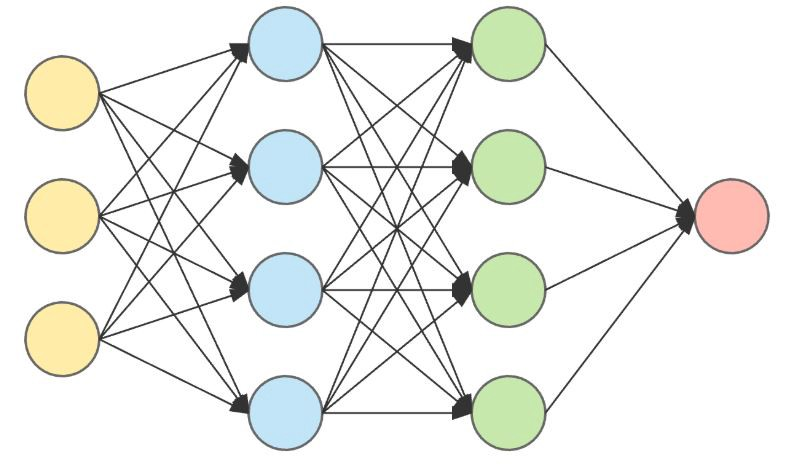
\includegraphics[scale=0.5]{front_image.jpeg}
    \end{center}
\end{titlepage}

\begin{document}
\raggedbottom
\begin{center}
    \small \textbf{Github}
    
    \vspace{0.2cm}
    
    \faGithub \ \small \href{https://github.com/dreilstad/FYS-STK3155/tree/master/Project1}{github.com/dreilstad/FYS-STK3155/Project1}
\end{center}
\vspace{0.5cm}
\section{Introduction}
Humans are incredible at using observations and relevant data to extract useful information. Whether it is to predict future events, understand current events, or recognize patterns. We still do not fully understand how the human brain works and how humans are able to do these things at such high accuracy compared to other species. In the age of computers and the internet, data has become an abundant and important resource. Due to the amount of data, it is necessary to automate the process of prediction, classification and/or pattern recognition. Humans are susceptible to mistakes, and machines are able to do computations significantly faster than humans. But how can machines achieve the same level of accuracy as humans?\\
\\
A method, initially hypothesized in the 1940s, called neural networks has recently become very popular and important in the machine learning field. A neural network is vaguely based on the biological neural networks in the human brain. The use of neural networks in prediction and classification problems has in many cases achieved great results. For example, an article\cite{skin} published in The Lancet compared the accuracy of humans versus machine-learning algorithms such as CNNs for classification of pigmented skin lesion. Convolutional Neural Networks (CNNs) is a type of neural network for images. The article found that the machine-learning classification algorithms outperformed even the most experienced human experts in the diagnosis of pigmented skin lesions.\\
\\
The focus of this project was to study regression and classification problems using different methods. For regression, linear regression methods and neural networks was used. For classification, neural networks and logistic regression was used and compared. Own code was implemented for neural networks and logistic regression, and code for linear regression was reused from project 1.\cite{project1} In addition the Stochastic Gradient Descent algorithm was studied and implemented, which is an important building block of the aforementioned methods. All code written for Stochastic Gradient Descent, neural networks and logistic regression can be found in the linked GitHub repository. \\
\\
The following sections of the report starts with an outline of the theory and method used for producing the results in the present work. Subsequently, information about the datasets used is provided. Afterwards the results are presented and discussed. The report concludes with the main findings of the project and future directions.
\section{Method}
This sections outlines the theory and method behind Stochastic Gradient Descent (SGD) as a building block for various regression methods, as well as neural networks. Different variants of SGD is also presented. Afterwards, the theory behind feed forward neural networks and logistic regression is defined.
\subsection{Stochastic Gradient Descent}
\subsubsection{Gradient Descent}
Gradient Descent is an iterative optimization algorithm for finding the minimum of a differentiable function. In our case, the function is the cost function which we want to minimize. Referring to Project 1\cite{project1} where various Regression methods was studied, we estimated the parameters of a vector named $\B$ such that the error of the model is minimized analytically.\\
\\
The gradient descent algorithm allows us to estimate such parameters iteratively. The algorithm starts with initializing the parameters with a starting value, with either zero values, random values or by a chosen distribution. Then the gradient of the cost function
$$
\nabla_{\beta} C(\B) = \sum_{i=1}^{n}\nabla_{\beta} c_{i}(\mathbf{x}_{i}, \B)
$$
with respect to the parameters of $\B$ is calculated. The gradient of a multi-variable function represents the direction and rate of fastest increase. Using the gradient, $\B$ is subtracted by $\eta\nabla C(\B)$. We subtract because we want to move in the direction of the minimum in order to minimize the cost function. For every step in the direction of the negative gradient, $\B$ is updated using equation (1)
\begin{align}
    \B_{i + 1} = \B_{i} - \eta \nabla_{\beta} C(\B)
\end{align}
for $i \geq 0$, and where $\eta$ is set to be a small value. The value of $\eta$ decides how large a step we move in the direction of the negative gradient towards a minimum. A value too large can cause us to overshoot the minimum and lead to a divergence from the minimum. A value too small leads to a slow convergence towards a minimum and a very large number of iterations is needed to converge. We want to tune $\eta$ such that the algorithm does not diverge but also convergences quickly enough. Tuning the learning rate $\eta$ is an essential problem when implementing gradient descent and variants of gradient descent.\\
\\
\begin{figure}[ht]
    \centering
    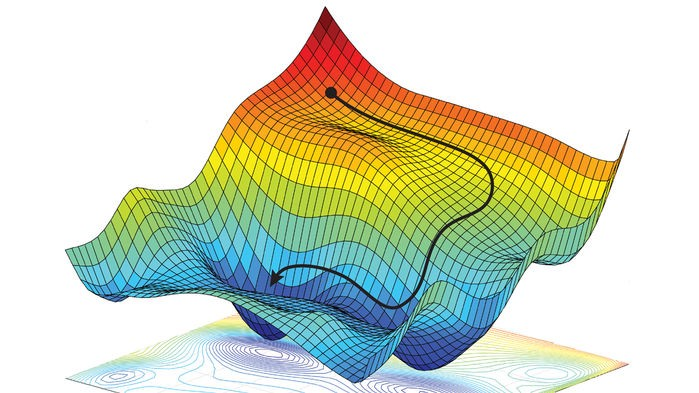
\includegraphics[width=\columnwidth]{sgd_example.jpeg}
    \caption{3D visualization of gradient descent. The model is dependent on two parameters and visualized in 3D space where the error from the cost function represents the z-axis in the figure. Source: \href{https://towardsdatascience.com/coding-deep-learning-for-beginners-linear-regression-gradient-descent-fcd5e0fc077d}{https://towardsdatascience.com/coding-deep-learning-for-beginners-linear-regression-gradient-descent-fcd5e0fc077d}}
    \label{fig:1}
\end{figure} \\
Figure \ref{fig:1} illustrates the optimization algorithm nicely even though the model only uses two parameters. Anymore parameters becomes difficult to visualize. An analogy often used, is to think of the cost function in Figure 1 as the terrain of a mountain or hill. At a given starting position you start walking in the steepest direction downhill for every step you take until you reach flat ground where you stop.\\
\\
As one can imagine, a problem arises when the function has several local minimum including a global minimum. How do we know if we have reached the bottom, i.e. the global minimum, and not a local minimum? A problem with gradient descent is that the algorithm is deterministic, meaning that the algorithm will in most cases converge on a local minimum when the cost function is varied and rugged. The performance of the algorithm can also be very sensitive to the starting conditions and also choice of learning rate, and is also very computationally expensive when using a large dataset because the algorithm has to sum over all datapoints when calculating the gradient. Stochastic gradient descent tries to solve some of the shortcomings of the gradient descent algorithm. 
\subsubsection{Stochastic approximation of gradient descent}
The underlying motivation behind SGD comes from gradient descent having to sum over all datapoints when calculating the gradient. As mentioned, this can become very computationally expensive. SGD solves this by randomly selecting subsets of the entire dataset, and applying the optimization algorithm on the subsets instead. The computational cost is significantly reduced, which is especially useful when dealing with problems and datasets with a high number of independent variables.\\
\\
The parameters of $\B$ is therefore updated for each iteration using equation (2)
\begin{align}
    \B_{i + 1} &= \B_{i} - \eta \sum_{i \in B_{k}}^{n}\nabla_{\beta} c_{i}(\mathbf{x}_{i}, \B)
\end{align}
where $B_{k}$ denotes the $k$'th minibatch. For $n$ datapoints and $M$ being the size of each minibatch, we have $\frac{n}{M}$ minibatches. The SGD algorithm iterates over each minibatch for $k = 1, . . ., \frac{n}{M}$, as opposed to the entire dataset with gradient descent. In addition, the algorithm typically iterates over the minibatches a specified number of epochs or until a minimum under a certain threshold has been reached. For this project, the former variant was implemented.\\
\\
While SGD improves the performance of the model significantly compared to gradient descent, there are several variants and extension that aims to improve SGD further. The variants presented are the ones implemented for the project, but there exists a plethora of other variants than the ones presented here.
\subsubsection{SGD variants}
\begin{center}
    \textbf{Decaying learning rate}
\end{center}
A different approach, instead of a fixed learning rate $\eta$, is to let $\eta$ depend on the number of epochs. The idea is to force $\eta$ smaller as the number of epochs becomes higher. 
\begin{align}
    \eta(t; t_{0}, t_{1}) = \frac{t_{0}}{t_{1} + t}
\end{align}
where $t_{0}$, $t_{1} > 0$ are fixed numbers and $t = e\cdot m + k$. $m$ is the number of minibatches, $e$ is current epoch number and $k$ is the $k$'th minibatch. The assumption is that as the number of epochs/iterations becomes higher, the algorithm will have approached the minimum and forcing the learning rate smaller makes sure the algorithm does not overshoot the minimum.
\begin{center}
    \textbf{RMSprop}
\end{center}
RMSprop is also a variant which computes an adaptive learning rate $\eta$, proposed by Geoff Hinton\cite{rmsprop}. The difference is that a  learning rate $\eta$ is specified beforehand as with standard SGD, but the learning rate is divided by the running squared average of the second moment of the gradient.
\begin{align*}
    \mathbf{g}_{i} &= \nabla_{\B}C(\B)\\
    \mathbf{s}_{i} &= \rho \mathbf{s}_{i-1} + (1 - \rho)\mathbf{g}_{i}^{2}\\
    \B_{i+1} &= \B_{i} - \eta\frac{\mathbf{g}_{i}}{\sqrt{\mathbf{s}_{i} + \epsilon}} \numberthis\label{eqn}
\end{align*}
Hinton proposes to set $\eta = 0.001$, $\rho = 0.9$ and $\epsilon \sim 10^{-8}$. The idea is to reduce the learning rate in the direction where the norm of the gradient is consistently large, but allows faster convergence with a larger learning rate in the case of saddle points where standard SGD often can get stuck and not converge quickly enough.
\begin{center}
    \textbf{ADAM}
\end{center}
ADAM is also an adaptive learning rate optimizer which combines RMSprop and SGD with momentum. ADAM also bias corrects the first and second moment of the gradient.\\
\begin{align*}
    \mathbf{g}_{i} &= \nabla_{\B}C(\B)\\
    \mathbf{m}_{i} &= \rho_{1} \mathbf{m}_{i-1} + (1 - \rho_{1})\mathbf{g}_{i}\\
    \mathbf{s}_{i} &= \rho_{2} \mathbf{s}_{i-1} + (1 - \rho_{2})\mathbf{g}_{i}^{2}\\
    \mathbf{\hat{m}}_{i} &= \frac{\mathbf{m}_{i}}{1 - \rho_{1}^{i}}\\
    \mathbf{\hat{s}}_{i} &= \frac{\mathbf{s}_{i}}{1 - \rho_{2}^{i}}\\
    \B_{i+1} &= \B_{i} - \eta\frac{\mathbf{\hat{m}}_{i}}{\sqrt{\mathbf{\hat{s}}_{i}} + \epsilon} \numberthis\label{eqn}
\end{align*}
The optimization method often performs very well while also being computationally efficient compared to other variants, and has become a very popular optimization algorithm. It was first proposed by Diederik P. Kingma \& Jimmy Lei Ba.\cite{ADAM}
\subsubsection{SGD with linear regression}
In project 1 for linear regression, the Mean Squared Error was used as the cost function.\cite{project1} Using SGD to find the parameters of $\B$ instead of matrix inversion, means calculating the gradient at each step. We can derive an analytical solution to the gradient for both OLS and Ridge regression. For OLS, the gradient is defined as
\begin{align}
    \nabla_{\beta} C^{OLS}(\B) = \frac{2}{n}\X^{T}(\X\B - \y)
\end{align}
For Ridge regession, which contains a regularization term, the gradient is defined as
\begin{align}
    \nabla_{\beta} C^{Ridge}(\B) = 2(\X^{T}(\X\B-\y)+\lambda\B)
\end{align}
where $\X$ is the design matrix presented in project 1.
\subsection{Multinomial Logistic Regression}
In project 1, the goal of linear regression was presented as fitting the parameters of $\B$ to a function in order to predict the outcome when applying the model on a set of independent variables. \\
\\
Logistic regression however, is a classification method used to predict the probabilities of different outcomes of a dependent variable when applied to a set of independent variables. Standard logistic regression deals with only a certain category or outcome. Meaning a binary problem, where for example binary logistic regression is used to predict yes/no on whether or not a person has cancer. In this project, the focus will be on multinomial logistic regression instead because of the dataset presented later in the report.\\
\\
Multinomial logistic regression is a generalization of logistic regression to several classes/categories/outcomes. It is used when the dependent variable is nomial, meaning that it falls into a set of categories which cannot be ordered together in any meaningful way. For example, which political party a person will vote for given certain demographic characteristics and personality traits.\\
\\
Multinomial logistic regression uses the softmax function. With $K$ classes, softmax function is defined as 
\begin{align}
    p_{k} = p(C = k|\mathbf{x}_{i};\B) = \frac{e^{\matbf{x_{i}}\B_{k}}}{\sum_{j = 1}^{K}e^{\matbf{x_{i}}\B_{j}}}
\end{align}
which represents the probability of class $k$ given input $\mathbf{x}_{i}$ and $\beta_{k}$ parameters for class $k$. The softmax function divides the probability of class $k$ by the sum of the probability of all $K$ possible classes.\\
\\
The cost function, also known as the cross-entropy, used with the softmax classifier function is defined as
\begin{align}
    C(\B) = -\sum_{i=1}^{K}y_{i}log(p_{i})
\end{align}
In order to use SGD to estimate $\B$ for the classes, we use the gradient of the cost function. The gradient can be compacted using vector and matrix multiplication. The gradient of the cost function can be shown to be written as
\begin{align}
    \nabla C(\B) = -\X^{T}(\y - \mathbf{p})
\end{align}
Since we are using SGD and minibatches, $\X$ will be a matrix of size $(n_{inputs}, n_{features})$, $\mathbf{y}$ is a matrix of size $(n_{inputs}, n_{categories})$ where the rows are so-called onehot vectors. A onehot vector contains a single $1$ element for the correct class or category and the remaining elements contains 0. $\mathbf{p}$ has the same size as $\y$, but each element in each row contains the probability of each class or category with the corresponding input. It is also convenient to scale the gradient with the size of the data, otherwise the magnitude of the gradient will make it necessary to tune the learning rate according to the amount for data. The gradient then becomes
\begin{align}
    \nabla C = -\frac{1}{n_{inputs}}\X^{T}(\y - \mathbf{p})
\end{align}
\subsection{Feed Forward Neural Networks}
\subsubsection{Feed forward}
A neural network is a collection of neurons ordered in one or more layers. The neurons receives input values which is the output from the previous layer and applies weights to the input in addition to a bias. The result is fed into an activation function and the output is passed to the neurons in the next layers. \\
\\
This type of information transfer neuron to neuron is based on the way biological neurons in the human brain function. Input is fed into the neural network and passes through the layers which in the end outputs a result which is dependent on the kind of problem we are solving. In this project, neural networks is tested on both regression problems and classification problems.\\
\\
The output $a$ of a single neuron with $n$ inputs from the previous layer is given by
\begin{align}
    a = f(\sum_{i = 1}^{n}w_{i}x_{i} + b_{i})
\end{align}
where $w_{i}$ is the weights, $x_{i}$ is the inputs and $f$ is the activation function. The general idea behind using an activation function, is that the weighted sum has to be over a certain threshold for the neuron to be considered "active" similar to how certain neruons in the brain are "active" when doing a task.\\
\\
There are several types of neural networks, such as Convolutional Neural Networks (CNNs) and Recurrent Neural Networks (RNNs), but the focus of this project is Feed Forward Neural Network (FFNNs).\\
\\
The first step for training the network is the feed forward pass. The feed forward pass of the neural network means we input our data into the first layer of neurons in the network. For each neuron in the layer, equation (12) is calculated. The result is saved as the input for the next layer. The same is done for the remaining layers, until we get an output. The output we get depends on the problem type, for example with classification the output would be the probabilites for each category or class.
\subsubsection{Backpropagation}
The next step is to optimize the weights and biases such that the error from output of the recent feed forward pass compared to the target values is minimized. This is the step where our neural network "learns". To optimize the weights and biases, we use the backpropagation algorithm.\\
\\
After doing a feed forward pass through the network, the algorithm goes backwards through the layers starting with the output layer. The error $\delta_{j}^{L}$ for the neurons in the last layer $L$, is calculated like this
\begin{align}
    \delta_{j}^{L} = f'(a_{j}^{L})\frac{\partial C}{\partial a_{j}^{L}}
\end{align}
where $j$ is the $j$'th neuron in layer $L$. Next is to continue going backwards through the hidden layers. The error $\delta_{j}^{l}$ for layer $l = L-1, L-2, ...$, is calculated like this
\begin{align}
    \delta_{j}^{l} = \sum_{k}\delta_{k}^{l+1}w_{kj}^{l+1}f'(a_{j}^{l})
\end{align}
The reason why the algorithm goes backwards through the layers is because we need the error from the next layer. The $\delta$ helps the network understand which neurons in the network should be penalized to reduce the error of the output. This we see in the final step of the backpropagation algorithm, which is updating the weights and biases using the errors calculated for each layer.\\
\\
The updating of the weights and biases is done using the SGD optimization algorithm presented earlier. The weights and biases are updated like this
\begin{align}
    w_{jk}^{l} &:= w_{jk}^{l} - \eta \delta_{j}^{l} a_{k}^{l - 1}\\
    b_{j}^{l} &:= b_{j}^{l} - \eta \delta_{j}^{l}
\end{align}
where $\delta_{j}^{l}a_{k}^{l - 1}$ in (15) is the derivative of the cost function w.r.t. to the weights $w_{jk}^{l}$ and likewise in (16) $\delta_{j}^{l}$ is the derivative w.r.t. the bias $b_{j}^{l}$. To improve the training of the neural network, a regularization parameter $\lambda$ is applied ot the weights. The regularization is done like this
\begin{align}
    w_{jk}^{l} &:= w_{jk}^{l} - \eta (\delta_{j}^{l} a_{k}^{l - 1} + \lambda w_{jk}^{l})
\end{align}
which can be rewritten to
\begin{align}
    w_{jk}^{l} &:= w_{jk}^{l} - \eta \delta_{j}^{l} a_{k}^{l - 1} - \eta \lambda w_{jk}^{l}\\
    w_{jk}^{l} &:= (1 - \eta\lambda)w_{jk}^{l} - \eta \delta_{j}^{l} a_{k}^{l - 1}
\end{align}
When training the neural network, the feed forward pass and the backpropagation step is repeated for each epoch and also using minibatches as the input. Stochastic Gradient Descent is the building block that allows the network to "learn".\\
\\
Backpropagation is essentially an algorithm for propogating the error back through the network and calculating the error each neuron is responsible for, and subsequently use this to update the weights and bias accordingly. If done enough number of epochs, you start to converge at a local minimum and approach the optimal weights and biases.
\subsubsection{Activation functions}
The activation function $f$ in equation (12) is a generalized notation. In fact there are several activation functions to choose from and the layers can also have different activation function depending on the problem type. For the regression case in this project, we use the an activation function for the hidden layers but no activation function for the output layer. In the the case of classification, we instead use the softmax function from equation (8) for the output layer.\\
\\
The activation functions for the hidden layers implemented and experimented with in this project is the Sigmoid function, tanh, RELU and Leaky RELU.
\begin{center}
    \textbf{Sigmoid}
\end{center}
The sigmoid function is defined as
\begin{align}
    \sigma(x) = \frac{e^{x}}{e^{x} + 1} = \frac{1}{1 + e^{-x}}
\end{align}
The function is defined for $\sigma(x) \in (0,1)$. The sigmoid is used in logistic regression for the binary case. The derivative is defined as
\begin{align}
    \frac{d}{dx}\sigma(x) = \sigma(x) \cdot (1 - \sigma(x))
\end{align}
\begin{center}
    \textbf{Tanh}
\end{center}
The hyperbolic tangent is defined as 
\begin{align}
    tanh(x) = \frac{sinh(x)}{cosh(x)} = \frac{e^{x} - e^{-x}}{e^{x} + e^{-x}}
\end{align}
The function is defined for $tanh(x) \in (-1, 1)$. The derivative is defined as
\begin{align}
    \frac{d}{dx}tanh(x) = 1 - tanh^{2}(x) = 1 - \frac{(e^{x} - e^{-x})^{2}}{(e^{x} + e^{-x})^{2}}
\end{align}
\begin{center}
    \textbf{RELU}
\end{center}
The RELU function is defined as 
\begin{align}
    RELU(x) &= x^{+} = max (0, x)\\
    RELU(x) &= \begin{cases} 
                    x, &\quad x > 0\\
                    0, &\quad x < 0
                \end{cases}
\end{align}
The derivative is defined as
\begin{align}
    \frac{d}{dx}RELU(x) = \begin{cases} 
                            1, &\quad x > 0\\
                            0, &\quad x < 0
                        \end{cases}
\end{align}
\begin{center}
    \textbf{Leaky RELU}
\end{center}
The Leaky RELU function is defined as 
\begin{align}
    LeakyRELU(x) &= \begin{cases} 
                    x, &\quad x > 0\\
                    0.01x, &\quad x < 0
                \end{cases}
\end{align}
The derivative is defined as
\begin{align}
    \frac{d}{dx}LeakyRELU(x) = \begin{cases} 
                                1, &\quad x > 0\\
                                0.01, &\quad x \leq 0
                                \end{cases}
\end{align}
\begin{figure}[ht]
    \centering
    \begin{subfigure}[b]{0.4\columnwidth}
        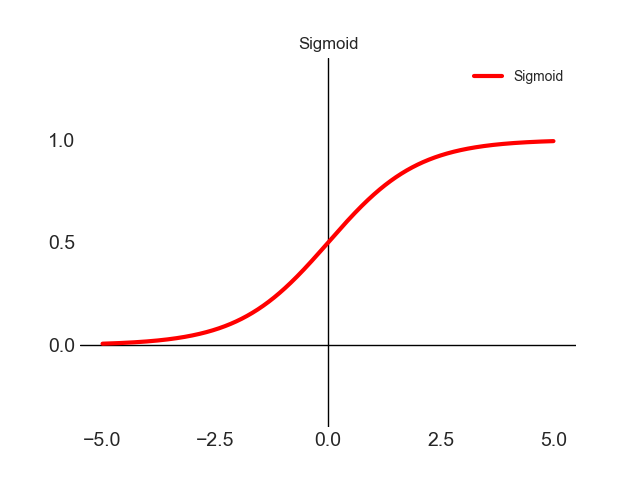
\includegraphics[width=\columnwidth]{Sigmoid_plot.png}
        \caption{Sigmoid}
    \end{subfigure}\hspace{0.1cm}
    \begin{subfigure}[b]{0.4\columnwidth}
        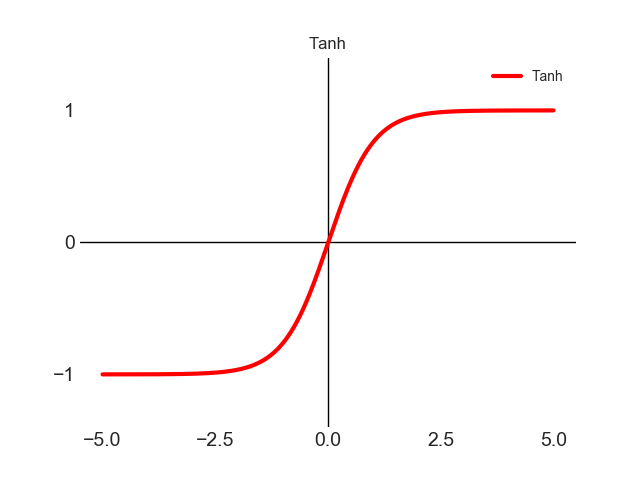
\includegraphics[width=\columnwidth]{Tanh_plot.png}
        \caption{Tanh}
    \end{subfigure}
    \vskip\baselineskip
    \begin{subfigure}[b]{0.4\columnwidth}
        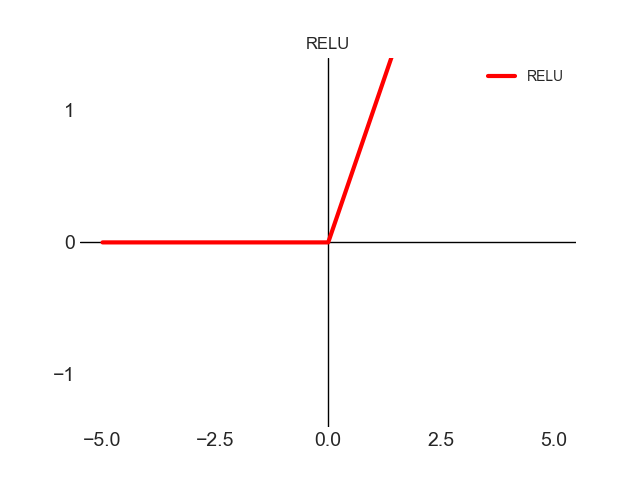
\includegraphics[width=\columnwidth]{relu_plot.png}
        \caption{RELU}
    \end{subfigure}\hspace{0.1cm}
    \begin{subfigure}[b]{0.4\columnwidth}
        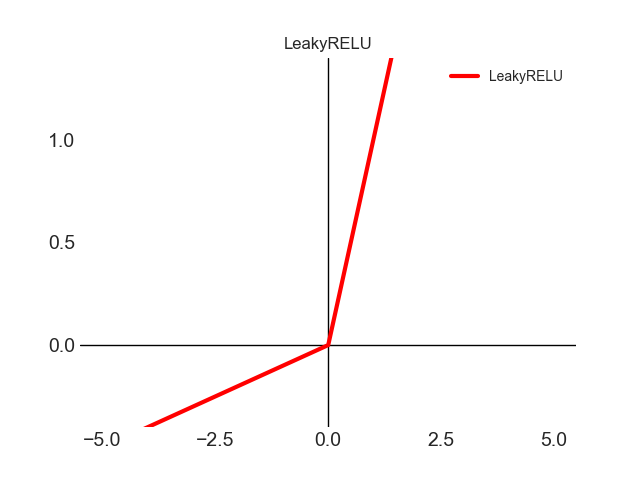
\includegraphics[width=\columnwidth]{leakyrelu_plot.png}
        \caption{LeakyRELU}
    \end{subfigure}
    \caption{Plot of the different activation functions.}
\end{figure}
\subsubsection{Weight initialization}
The way the weights in the neural network are initialized can greatly impact the performance of the model. When updating the weights using the stochastic gradient descent algorithm, a random initialization may lead to a slow convergence and ultimately to a "poorer" local minimum. \\
\\
In an article\cite{xavier} written by Xavier Glorot and Yoshua Bengio, they found that a model using the sigmoid function or the hyperbolic tangent as activation function performed poorly when using random initialization. They propose a new initialization scheme called normalized initialization instead, which they found lead to substantially faster convergence. The scheme is also called Xavier initialization. The Xavier initialization scheme is defined as
\begin{align}
    W \sim U\left[-\frac{6}{\sqrt{n_{j} + n_{j+1}}}, \frac{6}{\sqrt{n_{j} + n_{j+1}}}\right]
\end{align}
where $U$ is the uniform distribution in the interval and $n_{j}$ is number of neurons in the j'th layer.\\
\\
Another article\cite{he}, building on the previous article, found Xavier initialization not performing as well with the rectifiers such as RELU and Leaky RELU and proposes an improved initialization scheme called He initialization. The scheme is defined as
\begin{align}
    W \sim U\left[-\sqrt{\frac{2}{n_{j}}}, \sqrt{\frac{2}{n_{j}}}\right]
\end{align}
In this project, Xavier initialization is used when using the sigmoid or hyperbolic function as activation function. He initialization is used when using RELU or Leaky RELU as activation function.
\subsection{Model assessment and selection}
To accurately assess and select the best performing model, we need to use certain metrics for the different problem types. For regression, the Mean Squared Error is used. For classification, the accuracy score is used. The mentioned metrics are defined below, where $\ytilde$ is the prediction from the model.
\subsubsection{Accuracy score}
\begin{align}
        Accuracy(y, \widetilde{y}) &= \frac{1}{n} \sum_{i=0}^{n-1} I(y_{i} = \widetilde{y}_{i})
\end{align}
where $I$ is in indicator function. $1$ if $y = \widetilde{y}$, 0 if $y \neq \widetilde{y}$.
\subsubsection{Mean Squared Error}
\begin{align}
        MSE(y, \widetilde{y}) &= \frac{1}{n}\sum_{i=0}^{n-1}(y_{i} - \widetilde{y}_{i})^{2}
\end{align}
The Mean Squared Error (MSE) measures the quality of a predictor or estimator. The value from MSE is strictly positive. The closer the value is to 0, the more accurate the predictor/estimate is. The accuracy score is a metric for evaluating a classification model. The value from equation (31) is the fraction of predictions that was correct. An accuracy score of 1 means the model correctly predicted all samples.
\section{Datasets}
The datasets used in this project is the MNIST dataset of handwritten digits as images and also a generated dataset used with the Franke function. The MNIST dataset is used for classififcation when experimenting with the implementation of neural networks and multinomial logistic regression. The generated dataset with the Frank function is used for regression when testing the SGD variants and neural network implementation.
\subsubsection{Generated dataset with the Franke function}
See section 3 in project 1 for a more detailed explanation about the genereated dataset, and alos information about the Franke function.\cite{project1} 
\subsubsection{MNIST}
The MNIST database contains around 60,000 training images and 10,000 test images. In this project, a selection of approximately 1700 images from Scikit-Learn's dataset is used. The images are of size $8 \times 8$ with a handdrawn digit from $0-9$. Figure 2 shows an example image from the dataset.
\begin{figure}[ht]
    \centering
    
\includegraphics[scale=0.32]{mnist_example.png}
    \caption{Example image of handdrawn 0 from dataset.}
\end{figure}
\section{Results \& Discussion}
We start with testing and experimenting with Stochastic Gradient Descent, since it is the main building block of both logistic regression and neural network. The hyperparameters we can tune is the number of epochs, size of each minibatch, regularization parameter $\lambda$ and learning rate $\eta$. For SGD with learning rate decay, $t_{0}$ and $t_{1}$ can be adjusted.\\
\\
The hyperparameter that has the most impact on the performance of the model is the learning rate $\eta$. Figure \ref{fig:4} plots the MSE score as a function of the the learning rate $\eta$ on the generated dataset with the Franke function.\\
\begin{figure}[ht]
    \centering
    \begin{subfigure}[b]{0.9\columnwidth}
        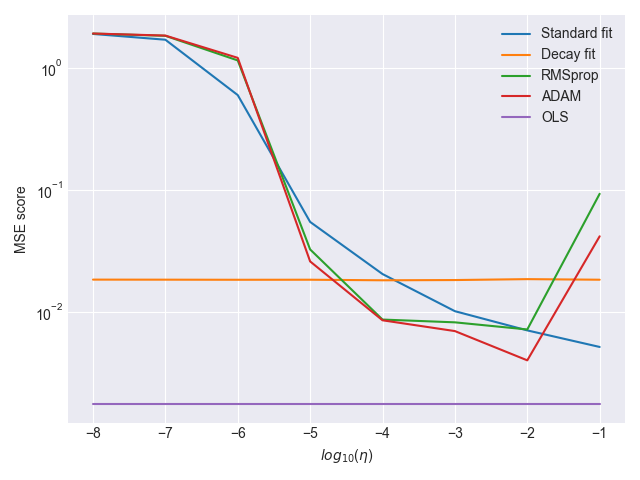
\includegraphics[width=\columnwidth]{compare_variants_learning_rates_Epochs=500_t0=5_t1=50_N=800_Noise=0.0_Degree=5.png}
        \caption{$N = 800$, noise $= 0.0$, epochs $= 500$, size of minibatch $= 1$, $t_{0} = 5$, $t_{1} = 50$ and polynomial degree $5$. Y-axis is logarithmically scaled.}
        \label{fig:4a}
    \end{subfigure}
    
    \begin{subfigure}[b]{0.9\columnwidth}
        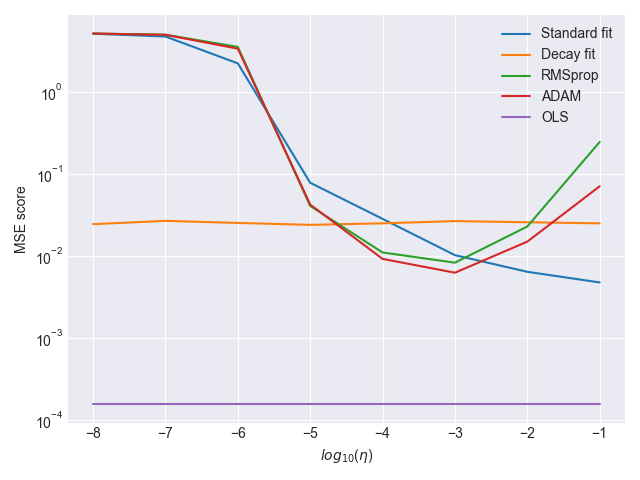
\includegraphics[width=\columnwidth]{compare_variants_learning_rates_Epochs=500_t0=5_t1=50_N=800_Noise=0.0_Degree=10.png}
        \caption{$N = 800$, noise $= 0.0$, epochs $= 500$, size of minibatch $= 1$, $t_{0} = 5$, $t_{1} = 50$ and polynomial degree $10$. Y-axis is logarithmically scaled.}
        \label{fig:4b}
    \end{subfigure}
    \caption{4(a) and 4(b) plots the MSE test score as a function of the learning rate $\eta$ with different level of complexity.}
    \label{fig:4}
\end{figure}\\
The common theme from figure \ref{fig:4a} and \ref{fig:4b} is that the error is minimized when the learning rate $\eta$ is within a certain interval. This interval is approximately $\eta \in [0.0001, 0.01]$. The result is logical. A learning rate $\eta$ too low will result in the step size towards the minimum to be too low and the algorithm does not converge quickly enough. A learning rate too high can result in overshooting the minimum and the algorithm may diverge.\\
\\
Also noticeable is that the RMSprop and ADAM optimizers has a much narrower interval where the model is acheives the best performance, while the standard SGD optimizer gradually achieves a better performance as the learning rate increases. Only studying figure \ref{fig:4}, it may suggest that the standard SGD optimizer generally perform better. The reason for this may be because the size of the minibatches was set to 1, meaning the whole training set is iterated. While this is possible for smaller datasets, for larger datasets this becomes computationally expensive and almost impossible. Figure \ref{fig:5} below, paints a different picture when increasing the size of the minibatches.
\begin{figure}[ht]
    \centering
    \begin{subfigure}[b]{0.9\columnwidth}
        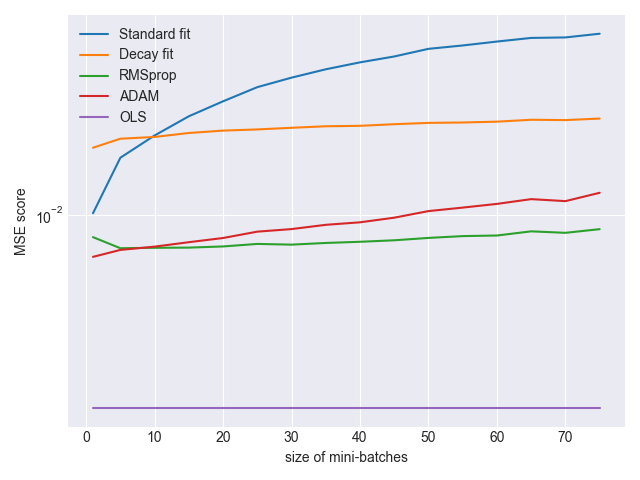
\includegraphics[width=\columnwidth]{compare_variants_minibatches_LR=0.001_Epochs=500_t0=5_t1=50_N=800_Noise=0.0_Degree=5.png}
        \caption{$N = 800$, noise $= 0.0$, epochs $= 500$, $\eta = 0.001$, $t_{0} = 5$, $t_{1} = 50$ and polynomial degree $5$. Y-axis is logarithmically scaled.}
        \label{fig:5a}
    \end{subfigure}
    
    \begin{subfigure}[b]{0.9\columnwidth}
        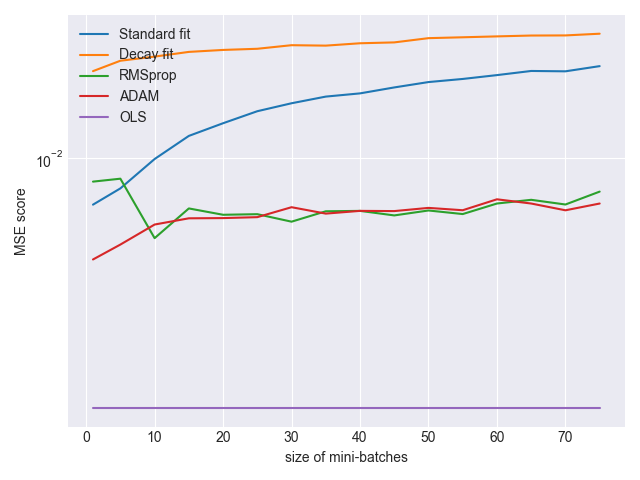
\includegraphics[width=\columnwidth]{compare_variants_minibatches_LR=0.01_Epochs=500_t0=5_t1=50_N=800_Noise=0.0_Degree=5.png}
        \caption{$N = 800$, noise $= 0.0$, epochs $= 500$, $\eta = 0.01$, $t_{0} = 5$, $t_{1} = 50$ and polynomial degree $5$. Y-axis is logarithmically scaled.}
        \label{fig:5b}
    \end{subfigure}
    \caption{5(a) and 5(b) plots the MSE test score as a function of the size of the minibatches.}
    \label{fig:5}
\end{figure}\\
Studying figures \ref{fig:5a} and \ref{fig:5b}, when the size of the minibatch is increased, the performance of standard SGD worsens. Meanwhile, RMSprop and ADAM only gradually increases as the size of the minbatches increases. Even when increasing learning rate to $\eta = 0.01$ in figure \ref{fig:5b}, the error is lower initially compared to \ref{fig:5a} but the error with standard SGD still increases. The benefit of being able to increase the size of the minibatches without the performance noticeably worsening is significant. Estimating $\B$ becomes much more computationally efficient.\\
\\
The reason why RMSprop and ADAM performs better, is because the two optimizers takes advantage of the moment of the gradient and this allows the algorithm to more quickly converge. A more rapid convergence with RMSprop and ADAM is also evident in figure \ref{fig:6}.
\begin{figure}[ht]
    \centering
    \begin{subfigure}[b]{0.87\columnwidth}
        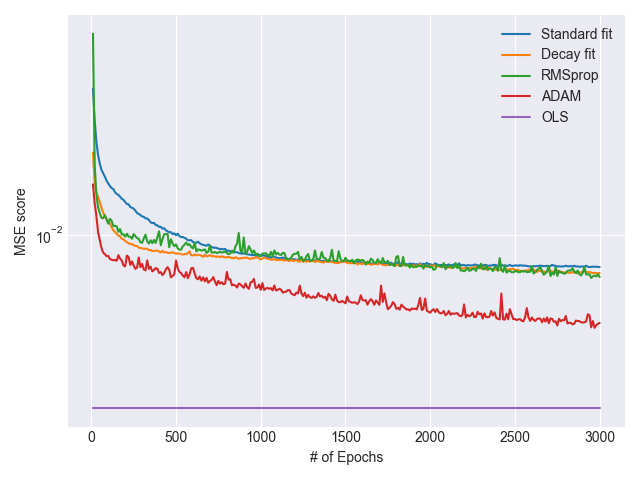
\includegraphics[width=\columnwidth]{compare_variants_epochs_LR=0.001_t0=5_t1=50_N=800_Noise=0.0_Degree=5.png}
        \caption{$N = 800$, noise $= 0.0$, size of minibatch $= 1$, $\eta = 0.001$, $t_{0} = 5$, $t_{1} = 50$ and polynomial degree $5$. Y-axis is logarithmically scaled.}
        \label{fig:6a}
    \end{subfigure}
    
    \begin{subfigure}[b]{0.87\columnwidth}
        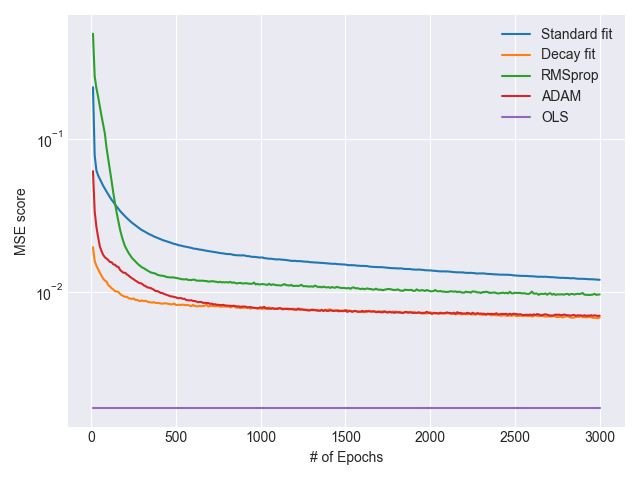
\includegraphics[width=\columnwidth]{compare_variants_epochs_LR=0.0001_t0=5_t1=50_N=800_Noise=0.0_Degree=5.png}
        \caption{$N = 800$, noise $= 0.0$, size of minibatch $= 1$, $\eta = 0.0001$, $t_{0} = 5$, $t_{1} = 50$ and polynomial degree $5$. Y-axis is logarithmically scaled.}
        \label{fig:6b}
    \end{subfigure}
    \caption{6(a) and 6(b) plots the MSE test score as a function of number of epochs.}
    \label{fig:6}
\end{figure}\\
From figures \ref{fig:6a} and \ref{fig:6b}, we can see from the curve that RMSprop and ADAM converges more quickly than standard SGD. Also comparing RMSprop and ADAM, the ADAM optimizer converges at a smaller error than RMSprop in both \ref{fig:6a} and \ref{fig:6b} for different learning rates. RMSprop converges at almost the same error as standard SGD but at around epoch $= 1000$ in \ref{fig:6a} and epoch $= 3000$ in \ref{fig:6b}. However comparing them in the interval $[0, 500]$, RMSprop converges quicker with less epochs.
\begin{figure}[ht]
    \centering
    \begin{subfigure}[b]{\columnwidth}
        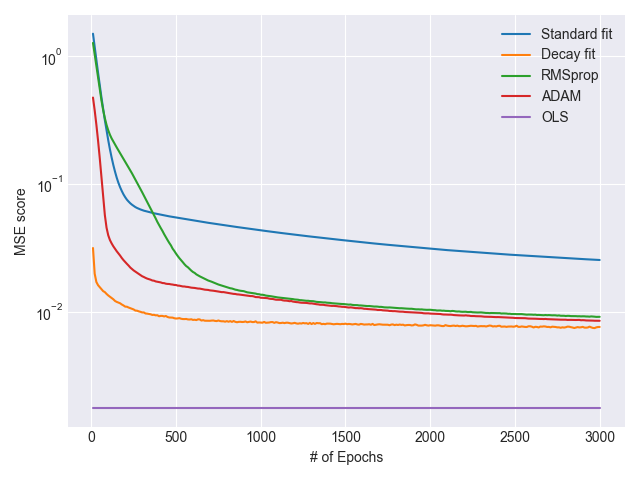
\includegraphics[width=\columnwidth]{compare_variants_epochs_MB=10_LR=0.0001_t0=5_t1=50_N=800_Noise=0.0_Degree=5.png}
        \caption{$N = 800$, noise $= 0.0$, size of minibatch $= 10$, $\eta = 0.0001$, $t_{0} = 5$, $t_{1} = 50$ and polynomial degree $5$. Y-axis is logarithmically scaled.}
    \end{subfigure}
    \caption{7(a) plots the MSE test score as a function of number of epochs.}
    \label{fig:7}
\end{figure}\\
However when increasing the size of the minibatches to 10 in figure \ref{fig:7}, we see that RMSprop converges at a much smaller error than standard SGD. Also noticeable from figure \ref{fig:7} is that while ADAM and RMSProp converges at the  same value, ADAM converges a lot quicker. The reason for this may be due to ADAM taking advantage of the first moment of the gradient and also bias-correcting. Therefore the ADAM optimizer may be able to more quickly get out of saddle points than RMSprop.\\
\\
Also performing well is SGD with decaying learning rate compared to RMSprop and ADAM, considering the simplicity of the variant. SGD with decay may perform worse for sparse datasets, but for the generated dataset with the Franke function it performs very well and converges very quick. In figure \ref{fig:6a} ADAM converges at a smaller value, meaning that ADAM may outperform SGD with decay if tuned correctly.\\
\\
Using SGD with decay does mean having to tune the two parameters $t_{0}, t_{1}$, instead of just the learning rate $\eta$. Still, it is the ratio $t_{0}/t_{1}$ that decides the initial learning rate. Plotting the MSE test score as a function of $t_{1}$ while holding $t_{0}$ constant, results in figure \ref{fig:8}.\\
\\
\begin{figure}[ht]
    \centering
    \begin{subfigure}[b]{0.9\columnwidth}
        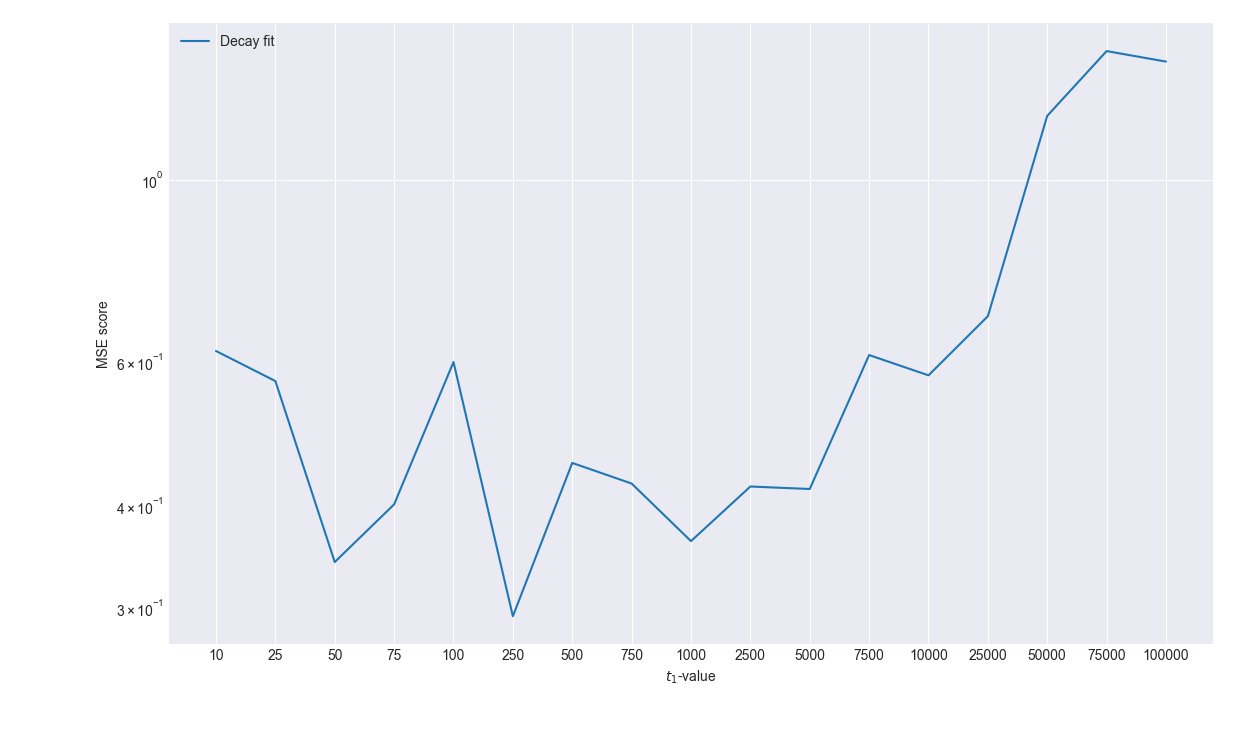
\includegraphics[width=\columnwidth]{decay_fit_learning_decay_t0=5Epochs=500_N=800_Noise=0.0_Degree=5.png}
        \caption{$N = 800$, noise $= 0.0$, size of minibatch $= 10$, epochs $= 500$, $t_{0} = 1$, and polynomial degree $5$. Y-axis is logarithmically scaled.}
    \end{subfigure}
    \caption{8(a) plots the MSE test score as a function of increasing $t_{1}$-value.}
    \label{fig:8}
\end{figure}\\
SGD with decay in figure \ref{fig:8} achieves the lowest error for $t_{1} = 250$, and also $t_{1} = 50$ not far off. Generally SGD with decay performs best with $t_{1} \in [10, 5000]$. A higher value than $5000$ results in a higher error. The reason for this is because the initial learning rate $\eta$ is too small at the start and for each epoch becomes smaller and smaller. This means the optimizer cannot converge quickly enough due to the small step size. In comparison, a smaller $t_{1}$ means that the optimizer at the beginning has a larger learning rate and therefore approaches a minimum faster initially. As the number of epochs increases the steps size towards the minimum decreases meaning there is less chance of overshooting the minimum.\\
\\
Moving on to Ridge regression, we must tune an additional hyperparameter. The optimal value for the regularization parameter $\lambda$, can be visualized by plottting a heatmap. Figure \ref{fig:9} shows the heatmap of the MSE test score plotted as a function of the learning rate $\eta$ and regularization parameter $\lambda$. A more red value means a lower MSE test score.
\begin{figure}[!ht]
    \centering
    \begin{subfigure}[b]{0.9\columnwidth}
        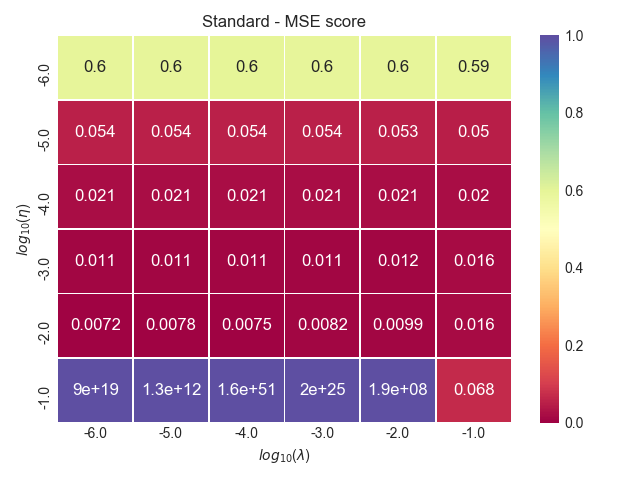
\includegraphics[width=\columnwidth]{lmbda_vs_lr_heatmap_Epochs=500_size_batch10_Variant=Standard_N=800_Noise=0.0_Degree=5_MSE.png}
        \caption{Standard SGD}
        \label{fig:9a}
    \end{subfigure}
    
    \begin{subfigure}[b]{0.9\columnwidth}
        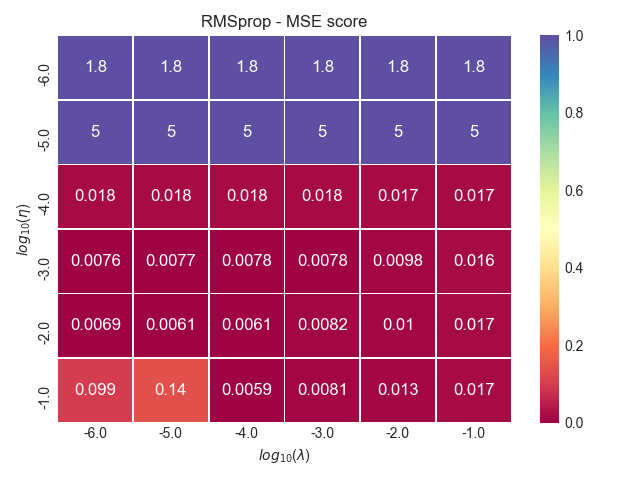
\includegraphics[width=\columnwidth]{lmbda_vs_lr_heatmap_Epochs=500_size_batch10_Variant=RMSprop_N=800_Noise=0.0_Degree=5_MSE.png}
        \caption{RMSprop}
        \label{fig:9b}
    \end{subfigure}
    
    \begin{subfigure}[b]{0.9\columnwidth}
        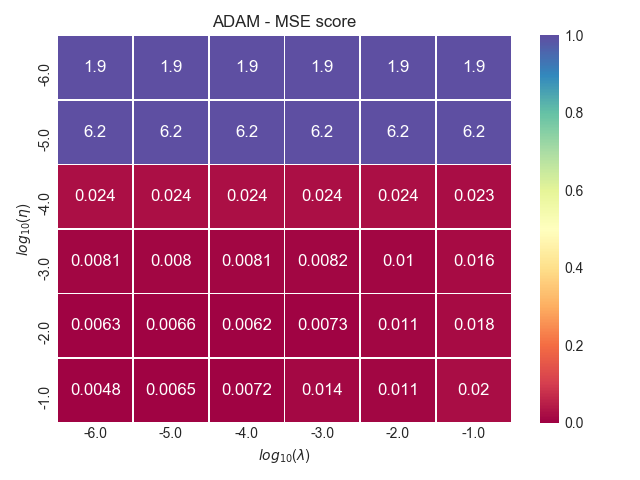
\includegraphics[width=\columnwidth]{lmbda_vs_lr_heatmap_Epochs=500_size_batch10_Variant=ADAM_N=800_Noise=0.0_Degree=5_MSE.png}
        \caption{ADAM}
        \label{fig:9c}
    \end{subfigure}
    \caption{9(a), 9(b) and 9(c) plots the MSE test score as a function of the learning rate $\eta$ and the regularization parameter $\lambda$. $N=800$, noise $= 0.0$, size of minibatch $= 10$, epochs $= 500$ and polynomial degree $5$.}
    \label{fig:9}
\end{figure}
\newpage
\noindent Studying figure \ref{fig:9a}, standard SGD achieves a minimum error of $0.0072$ for $\eta = 0.01$ and $\lambda = 1\cdot10^{-6}$. While RMSprop and ADAM achieves a minimum error of $0.0059$ and $0.0048$ respectively, with learning rate $\eta = 0.1$ with $\lambda = 1\cdot10^{-4}$ and $\lambda = 1\cdot10^{-6}$ in figures \ref{fig:9b} and \ref{fig:9c}.\\
\\
Generally RMSprop performs best within the interval $\eta \in [0.001, 0.01]$ and $\lambda \in [1\cdot10^{-6}, 1\cdot10^{-3}]$ and ADAM performs best within the interval $\eta \in [0.001, 0.1]$ and $\lambda \in [1\cdot10^{-6}, 1\cdot10^{-4}]$. However standard SGD really only achieves the same magnitude of error values for $\eta = 0.01$, indicating that RMSprop and ADAM requires less fine tuning of the parameters.\\
\\
As was mentioned when introducing RMSprop and ADAM, these optimizers utilizes an adaptive learning rate. Compared to standard SGD, the MSE test scores are a lot more stable across the heatmap. In \ref{fig:9a} for standard SGD with $\eta = 0.1$, the learning rate is too high meaning the gradient "blows up" and results in large errors.
\begin{figure*}[!b]
    \centering
    \begin{subfigure}[b]{\columnwidth}
        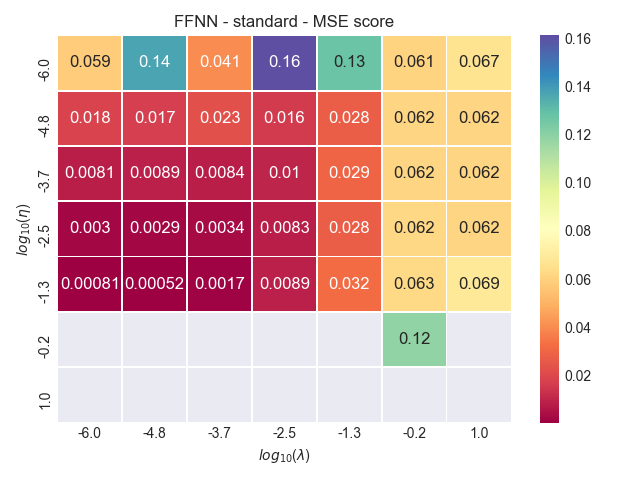
\includegraphics[width=1.1\columnwidth, height=0.65\columnwidth]{ffnn_heatmap_lmbda_vs_lr_Act=sigmoid_Epochs=1000_sizeMB=20_neurons=12_hl=1_Variant=FFNN - standard_N=800_Noise=0.0_Degree=5_MSE.png}
        \caption{Sigmoid activation function. 1 hidden layer, 12 neurons.}
        \label{fig:10a}
    \end{subfigure}\hspace{0.1cm}
    \begin{subfigure}[b]{\columnwidth}
        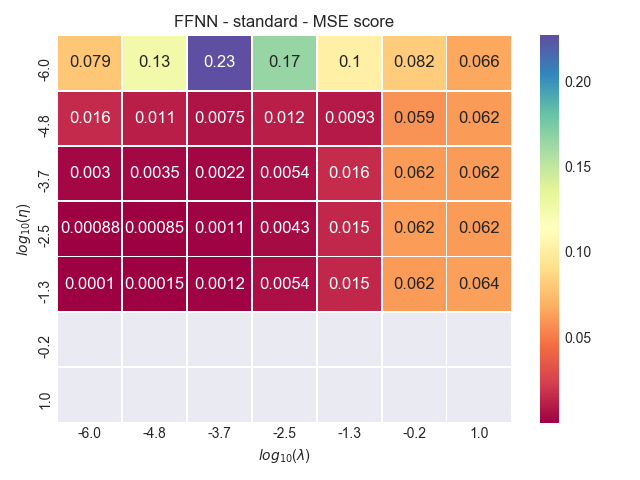
\includegraphics[width=1.1\columnwidth, height=0.65\columnwidth]{ffnn_heatmap_lmbda_vs_lr_Act=tanh_Epochs=1000_sizeMB=20_neurons=12_hl=1_Variant=FFNN - standard_N=800_Noise=0.0_Degree=5_MSE.png}
        \caption{tanh activation function. 1 hidden layer, 12 neurons.}
        \label{fig:10b}
    \end{subfigure}
    \vskip\baselineskip
    \begin{subfigure}[b]{\columnwidth}
        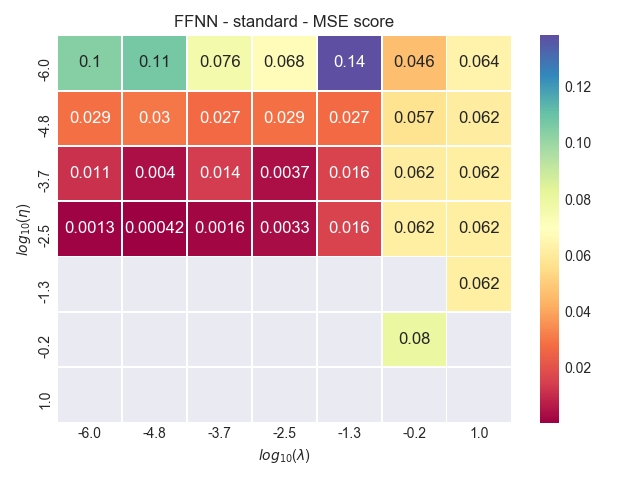
\includegraphics[width=1.1\columnwidth, height=0.65\columnwidth]{ffnn_heatmap_lmbda_vs_lr_Act=relu_Epochs=1000_sizeMB=20_neurons=12_hl=1_Variant=FFNN - standard_N=800_Noise=0.0_Degree=5_MSE.png}
        \caption{RELU activation function. 1 hidden layer, 12 neurons.}
        \label{fig:10c}
    \end{subfigure}\hspace{0.1cm}
    \begin{subfigure}[b]{\columnwidth}
        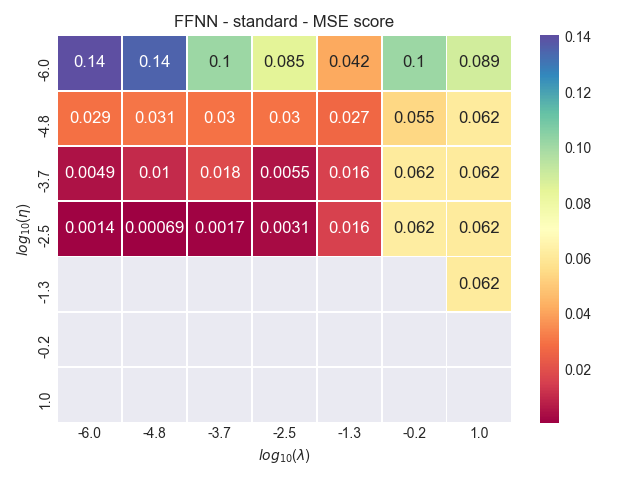
\includegraphics[width=1.1\columnwidth, height=0.65\columnwidth]{ffnn_heatmap_lmbda_vs_lr_Act=leakyrelu_Epochs=1000_sizeMB=20_neurons=12_Variant=FFNN - standard_N=800_Noise=0.0_Degree=5_MSE.png}
        \caption{LeakyRELU activation function. 1 hidden layer, 12 neurons.}
        \label{fig:10d}
    \end{subfigure}
    \captionsetup{width=2\columnwidth}
    \caption{Figures 10 plots the MSE test score as a function of the learning rate $\eta$ and the regularization parameter $\lambda$ with different activation functions. $N=800$, noise $= 0.0$, size of minibatch $= 20$, epochs $= 1000$ and polynomial degree $5$. }
    \label{fig:10}
\end{figure*}\\
\\
Next we use SGD to train a neural network on the same dataset. Starting with a feed forward neural network consisting of 1 hidden layer with 12 neurons. Figure \ref{fig:10} plots the MSE test score as a function of the learning rate $\eta$ and regularization parameter. Missing values means that either training caused overflow due to "exploding" gradient or "vanishing" gradients, or the error value was over a certain threshold. In this case, the threshold was was 10.\\
\\
Studying figure \ref{fig:10}, we see the neural network is able to achieve a low error on the test set for all activation functions. Figures \ref{fig:10a} and \ref{fig:10b} show the sigmoid and tanh function generally performing better for a larger range of learning rates. While figures \ref{fig:10c} and \ref{fig:10d} show RELU and Leaky RELU only achieving the same error values for $\eta = 1\cdot 10^{-2.5}$, while also having missing values for $\eta = 1\cdot 10^{-1.3}$ when the sigmoid and tanh does not.\\
\\
Compared to Ordinary Least Squares and Ridge regression from project 1 with the same level of complexity, amount of data and noise. OLS and Ridge regression achieves the MSE test scores listed  in table \ref{tab:1}.
\begin{table}[h]
    \centering
    \caption{Minimum MSE test scores for OLS and Ridge regression. K-fold cross validation used as resampling technique with k-folds $= 10$. See project 1 for info on resampling technique.}
    \label{tab:1}
    \begin{tabular}{|c||c|c|c|}
    \hline
        Method & Degree & $\lambda$ & MSE test \\ 
        \hline\hline
        OLS & 5 & - & $0.001312$ \\ 
        \hline
        Ridge & 5 & $1\cdot 10^{-6.0}$ & $0.001313$ \\
        \hline
    \end{tabular}
\end{table}
Comparing table \ref{tab:1} and figures \ref{fig:10}, the neural network is able to achieve a lower error compared to using linear regression. For the neural network using tanh as activation function, the minimum MSE test error achieved is 0.0001 for $\eta = 1\cdot 10^{-1.3}$ and $\lambda = 1\cdot 10^{-6.0}$. The neural network is able to converge at an error 10 times lower than with linear regression. The reason for this is because neural networks have adaptability to highly non-linear functions and is able to generalize enough to not overfit.\\
\\
Similar results was found in a research article comparing multiple linear regression and neural networks for modeling concrete dam deformation\cite{lrvsffnn}. The function attempted to model in the article is also highly non-linear.\\
\\
Important to note is that training the neural network took considerably more time than fitting OLS and Ridge regression. So if training time is crucial and limited, linear regression is a better option than using neural networks. However if you want to achieve the lowest error possible, neural networks outperforms linear regression on the generated dataset with the Franke function.\\
\\
While standard SGD with neural networks is able to achieve low errors, the results in figure \ref{fig:10} are quite uneven for different learning rates and also has several missing values due to high error or exploding/vanishing gradients. Previously we found the ADAM optimizer to be more stable for a larger range of learning rates and also with size of minibatches larger than 1. In figure \ref{fig:11} below, with the exact same parameters used in figure \ref{fig:10}, the MSE test score is plotted as a function of the learning rate and regularization parameter where the ADAM optimizer is used instead of standard SGD.\\
\\
Studying figure \ref{fig:11}, we can see a considerable improvement compared to figure \ref{fig:10}. For all activation functions the range of learning rates $\eta$ where the neural network performs well is larger. This means the network requires much less fine tuning of the parameters to achieve an acceptable error value. This confirms the results found earlier when only  testing the SGD variants.\\
\\
Generally from studying figure \ref{fig:11}, when the regularization parameter $\lambda \geq 1\cdot 10^{-1.3}$ the MSE test error becomes $> 1\cdot 10^{-2}$. This is due to the regularization parameter preventing the neural network from changing the weights enough and therefore from converging quickly enough. The neural network achieving the lowest error is the one using tanh as activation function. In figure \ref{fig:11b}, the neural network converges at MSE test error $= 9.3\cdot 10^{-5}$ for $\eta = 1\cdot 10^{-3.7}$ and $\lambda = 1\cdot 10^{-6.0}$. The reason why tanh generally performs better than sigmoid is because it is centered around 0, while the sigmoid is centered around 0.5. Due to tanh being centered around 0 and being defined for $[-1, 1]$, the derivatives will be higher compared to sigmoid. Higher derivatives means the neural network learns faster and is less likely to get stuck during training at a "poor" local minimum. \\
\\
In figure \ref{fig:11c} where RELU is used as activation function, the neural network generally performs well. Comparing the performance of RELU to tanh, we see both achieving similar error scores but for a higher learning rate $\eta = 1\cdot 10^{-0.2}$ RELU outperforms both tanh and the rest. The sigmoid and tanh is susceptible to vanishing gradients when approaching a minimum which means the gradient becomes so small that the weights no longer updates and therefore the network does not learn. RELU does not suffer from this problem, and is the reason why it is currently widely used as activation function.\\
\\
While Leaky RELU is meant to prevent the "dying" RELU problem, in the case of the generated dataset with Franke function this does not have an impact. The "dying" RELU problem is when RELU always have values less than 0 which prevents the neural network from learning due to the gradient being 0 for negative values. Leaky RELU performs well similarly to RELU except for $\eta = 1 \cdot 10^{-0.2}$.\\
\\
The reason why the advantage of Leaky RELU does not impact the results is because of the way the weights are initialized. Leaky RELU is preferable and can perform better when you do not use a specific initialization scheme. When using random initialization with RELU, the neural network could end up stuck and not learn anymore.
\begin{figure*}
    \centering
    \begin{subfigure}[b]{\columnwidth}
        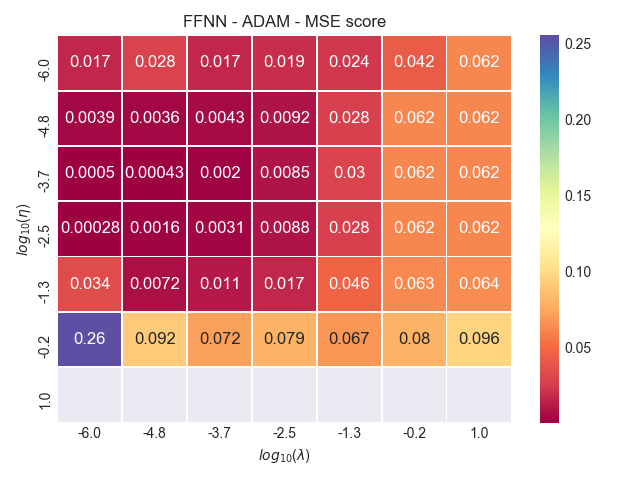
\includegraphics[width=1.1\columnwidth, height=0.65\columnwidth]{ffnn_heatmap_lmbda_vs_lr_Act=sigmoid_Epochs=1000_sizeMB=20_neurons=12_Variant=FFNN - ADAM_N=800_Noise=0.0_Degree=5_MSE.png}
        \caption{Sigmoid activation function. 1 hidden layer, 12 neurons.}
        \label{fig:11a}
    \end{subfigure}\hspace{0.1cm}
    \begin{subfigure}[b]{\columnwidth}
        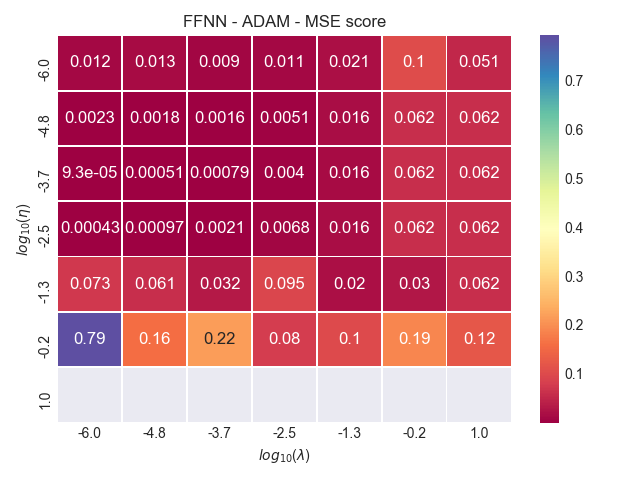
\includegraphics[width=1.1\columnwidth, height=0.65\columnwidth]{ffnn_heatmap_lmbda_vs_lr_Act=tanh_Epochs=1000_sizeMB=20_neurons=12_Variant=FFNN - ADAM_N=800_Noise=0.0_Degree=5_MSE.png}
        \caption{tanh activation function. 1 hidden layer, 12 neurons.}
        \label{fig:11b}
    \end{subfigure}
    \vskip\baselineskip
    \begin{subfigure}[b]{\columnwidth}
        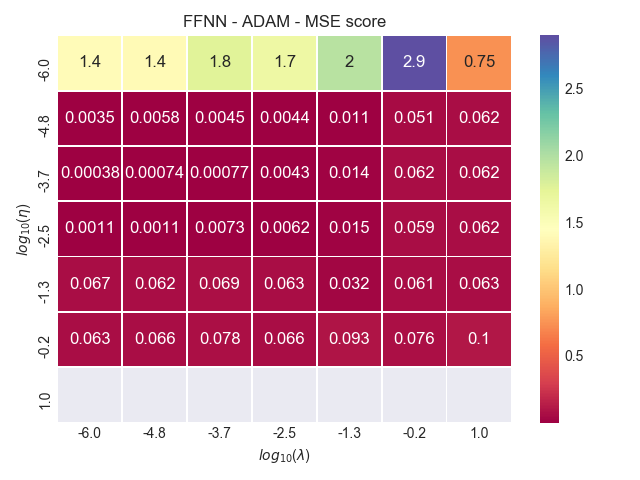
\includegraphics[width=1.1\columnwidth, height=0.65\columnwidth]{ffnn_heatmap_lmbda_vs_lr_Act=relu_Epochs=1000_sizeMB=20_neurons=12_Variant=FFNN - ADAM_N=800_Noise=0.0_Degree=5_MSE.png}
        \caption{RELU activation function. 1 hidden layer, 12 neurons.}
        \label{fig:11c}
    \end{subfigure}\hspace{0.1cm}
    \begin{subfigure}[b]{\columnwidth}
        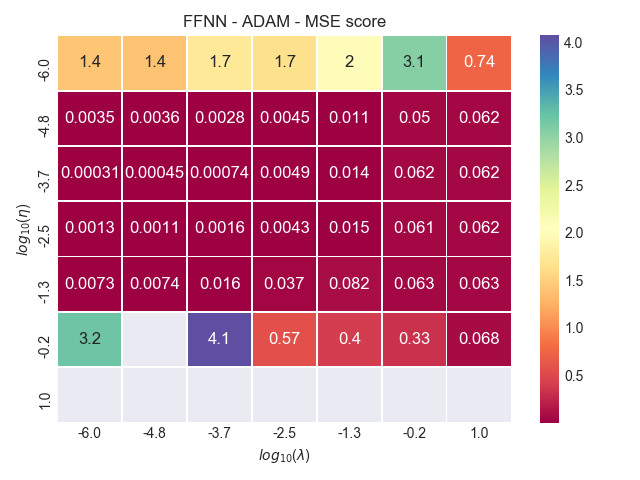
\includegraphics[width=1.1\columnwidth, height=0.65\columnwidth]{ffnn_heatmap_lmbda_vs_lr_Act=leakyrelu_Epochs=1000_sizeMB=20_neurons=12_Variant=FFNN - ADAM_N=800_Noise=0.0_Degree=5_MSE.png}
        \caption{LeakyRELU activation function. 1 hidden layer, 12 neurons.}
        \label{fig:11d}
    \end{subfigure}
    \captionsetup{width=2\columnwidth}
    \caption{Figures 10 plots the MSE test score as a function of the learning rate $\eta$ and the regularization parameter $\lambda$ with different activation functions. $N=800$, noise $= 0.0$, size of minibatch $= 20$, epochs $= 1000$ and polynomial degree $5$. }
    \label{fig:11}
\end{figure*}\\
\\
Next we test the neural network on a classification problem. We use the images from the MNIST database. Start by studying the effect of changing the architecture of the neural network. Figure \ref{fig:12a} plots the accuracy as a function of the number of neurons in a single hidden layer neural network.
\begin{figure}[ht]
    \centering
    \begin{subfigure}[b]{\columnwidth}
        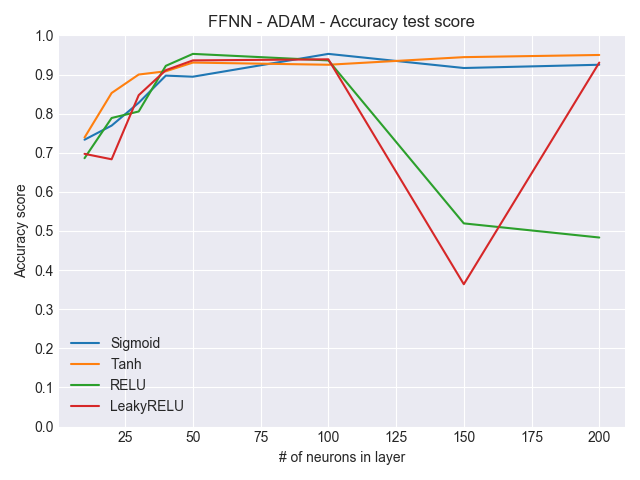
\includegraphics[width=\columnwidth]{ffnn_accuracy_vs_neurons_Epochs=200_sizeMB=50_variant=ADAM_lr=1e-05_lmbda=1e-05.png}
        \caption{Epochs $= 200$, size of minibatch $= 50$, $\eta = 0.00001$ and $\lambda = 0.00001$.}
    \end{subfigure}
    \caption{12(a) plots the accuracy score on the test set as a function of the number of neurons in a neural network constisting of a single hidden layer. ADAM optimizer used for training. Accuracy test score for number of neurons $\in [10, 20, 30, 40, 50, 100, 150, 200]$}
    \label{fig:12a}
\end{figure}\\
\\
Studying figure \ref{fig:12a}, we can see that the accuracy score up until neurons $= 100$ converges at 0.93 or 0.94. For a low amount of neurons, the neural network does not have the ability to capture all the necessary characteristcs. As the number of neurons increases, the accuracy test score converges to above 0.9. The increased amount of neurons enables the neural network to capture the necessary characteristics and therefore make more accurate predictions.\\
\\
For neurons $= 150$ we see a spike downwards in the accuracy when using RELU and Leaky RELU as activation function. The reason for this could be due to overfitting. There may be a point at which increasing the number of neurons only makes the neural network overfit to the training set. However seeing as sigmoid and tanh does not suffer the same dip, another explanation could simply be that the optimal learning rate $\eta$ and regularization parameter $\lambda$ are different for the rectifiers. The values used in figure \ref{fig:12a} could be more optimal for the sigmoid and tanh function.\\
\\
Next we study the effect of increasing the number of hidden layers in the neural network. Figure \ref{fig:13a} plots the accuracy test score as a function of the number of hidden layers, with each layer containing 50 neurons.\\
\\
Studying figure \ref{fig:13a}, the accuracy test score decreases when increasing the number of hidden layers for all activation functions except tanh. The reason for this is overfitting. Already for a single hidden layer with 50 neurons, the necessary and important characteristics are captured. Adding more hidden layers to the network results in overfitting to the training data.
\begin{figure}[ht]
    \centering
    \begin{subfigure}[b]{\columnwidth}
        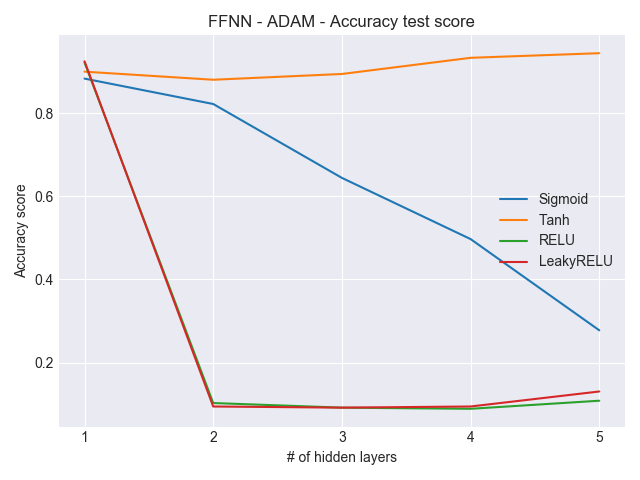
\includegraphics[width=\columnwidth]{ffnn_accuracy_vs_layers_Neurons=50_Epochs=200_sizeMB=50_variant=ADAM_lr=1e-05_lmbda=1e-05.png}
        \caption{Epochs $= 200$, size of minibatch $= 50$, $\eta = 0.00001$ and $\lambda = 0.00001$.}
    \end{subfigure}
    \caption{13(a) plots the accuracy score on the test set as a function of the number of hidden layers in a neural network. Each hidden layer contains 50 neurons. ADAM optimizer used for training.}
    \label{fig:13a}
\end{figure}\\
\\
The exception is the neural network using tanh as activation function, which achieves an accuracy score of 0.95 for 5 hidden layers. In both figure \ref{fig:12a} and figure \ref{fig:13a}, tanh as activation function in the neural network achieves the best accuracy score. This result is corroborated by the results in figure \ref{fig:14}.\\
\\
Comparing the results for each activation function in figure \ref{fig:14}, tanh as activation in the neural networks is able to consistently achieve an accuracy test score above 0.9 for almost all learning rates $\eta$ and regularization parameters $\lambda$. Tanh also achieve the highest accuracy score of 0.95, while the rest achieve a maximum accuracy score of 0.93.\\
\\
Neural networks with RELU and Leaky RELU are able to achieve a high accuracy score but for several combinations of learning rates $\eta$ and regularization parameter $\lambda$ the accuracy is significantly worse. For the MNIST dataset, RELU and Leaky RELU requires more fine tuning to find the optimal parameters. Still, tanh as activation function results in a consistently higher accuracy score compared to the rest with the current dataset, neural network architecture and parameters.
\begin{figure*}[ht]
    \centering
    \begin{subfigure}[b]{\columnwidth}
        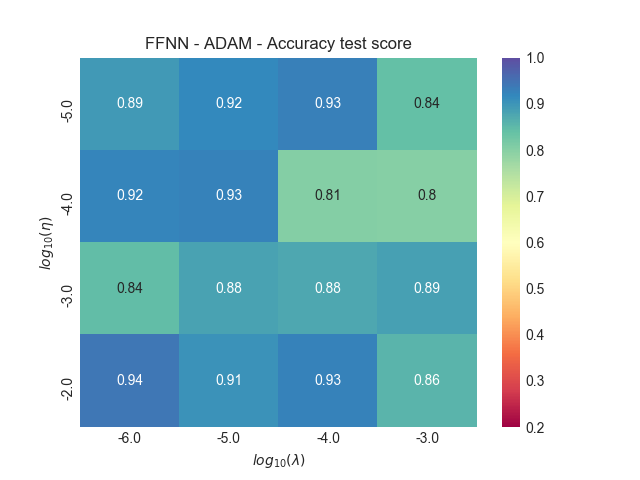
\includegraphics[width=1.1\columnwidth, height=0.65\columnwidth]{ffnn_accuracy_lr_vs_lmbda_act=sigmoid_Epochs=200_sizeMB=50_variant=ADAM.png}
        \caption{Sigmoid activation function. 1 hidden layer, 50 neurons.}
        \label{fig:14a}
    \end{subfigure}\hspace{0.1cm}
    \begin{subfigure}[b]{\columnwidth}
        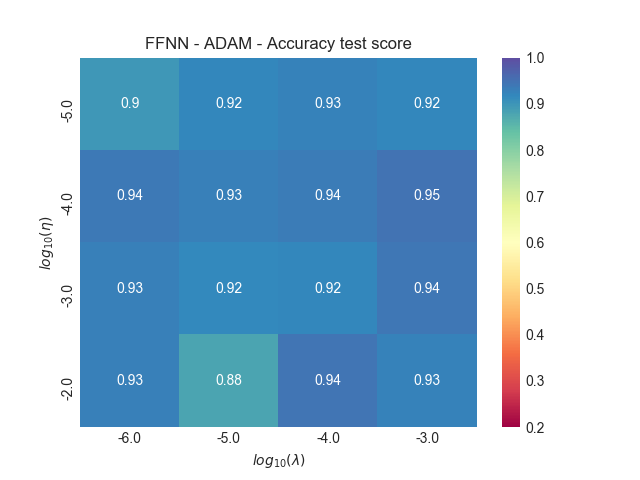
\includegraphics[width=1.1\columnwidth, height=0.65\columnwidth]{ffnn_accuracy_lr_vs_lmbda_act=tanh_Epochs=200_sizeMB=50_variant=ADAM.png}
        \caption{tanh activation function. 1 hidden layer, 50 neurons.}
        \label{fig:14b}
    \end{subfigure}
    \vskip\baselineskip
    \begin{subfigure}[b]{\columnwidth}
        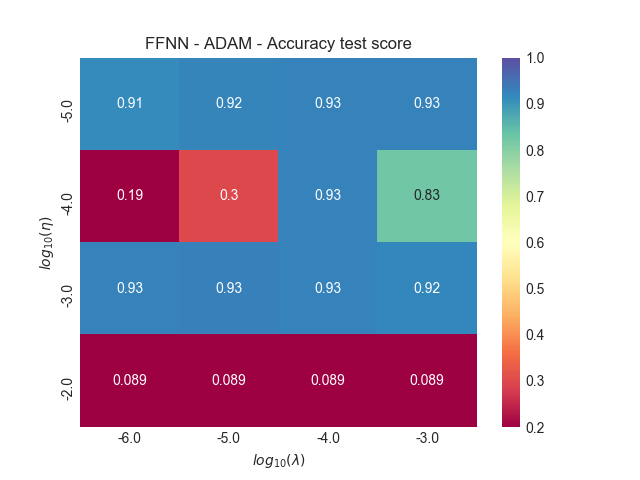
\includegraphics[width=1.1\columnwidth, height=0.65\columnwidth]{ffnn_accuracy_lr_vs_lmbda_act=relu_Epochs=200_sizeMB=50_variant=ADAM.png}
        \caption{RELU activation function. 1 hidden layer, 50 neurons.}
        \label{fig:14c}
    \end{subfigure}\hspace{0.1cm}
    \begin{subfigure}[b]{\columnwidth}
        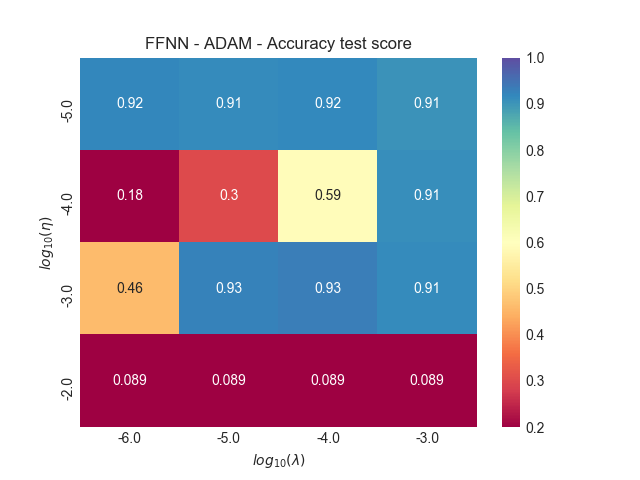
\includegraphics[width=1.1\columnwidth, height=0.65\columnwidth]{ffnn_accuracy_lr_vs_lmbda_act=leakyrelu_Epochs=200_sizeMB=50_variant=ADAM.png}
        \caption{LeakyRELU activation function. 1 hidden layer, 50 neurons.}
        \label{fig:14d}
    \end{subfigure}
    \captionsetup{width=2\columnwidth}
    \caption{Figures 14 plots the accuracy test score as a function of the learning rate $\eta$ and the regularization parameter $\lambda$ with different activation functions. Size of minibatch $= 50$ and epochs $= 200$. All subplots have the same color-scaling range.}
    \label{fig:14}
\end{figure*}\\
\\
Next we compare the results for neural networks in figure \ref{fig:14} to the results from logistic regression on the dataset in figure \ref{fig:15}. Figure \ref{fig:15} plots the accuracy score as a function of the learning rate $\eta$ and regularization parameter $\lambda$.\\
\\
From figure \ref{fig:15} we see both our own logistic regression code and Scikit's achieving a high accuracy test score. Own logistic regression performs slightly better than Scikit's for almost all $\eta$ and $\lambda$ values achieving a maximum accuracy score of 0.96 with $\eta = 0.1$. Scikit's SGDClassifier achives a maximum accuracy test score of 0.94.\\
\\
Compared to neural networks with sigmoid and tanh as activation function in figure \ref{fig:14}, the results are very similar. This is logical seeing as a neural network with one hidden layer using sigmoid as activation function is almost equivalent to logistic regression. The only difference is that the neural network uses the softmax function for the output layer.\\
\\
Logistic regression consistently outperforms neural networks using RELU or Leaky RELU as activation function for all $\eta$ and $\lambda$ values, and is on par with neural networks using sigmoid or tanh as activation function. The reason for this is likely due to the classification problem being quite simple. The images used are grayscale images with a total of 64 pixels. The important characteristics needed to accurately predict the number is less complex compared to other datasets and classification problems. As mentioned earlier with regression, neural networks has the advantage of being able to adapt to more complex and non-linear functions. For this reason, neural networks could likely outperform logistic regression for a more complex classification problem due to adaptability and generalizing enough to not overfit.\\
\\
In this case, logistic regression outperforms neural networks. A disadvantage with using neural networks is that it is quite computationally expensive to train, and if you want to use a more complex architecture you need more training data and training time. Logistic regression took significantly less time to train and was able to achieve the same level of accuracy. Another explanation as to why the nueral network performed worse or only on par with logistic regression could be due to the choice of architecture. The architecture chosen for the neural network could be suboptimal and changing it could improve the performance. 
\begin{figure*}[ht]
    \centering
    \begin{subfigure}[b]{\columnwidth}
        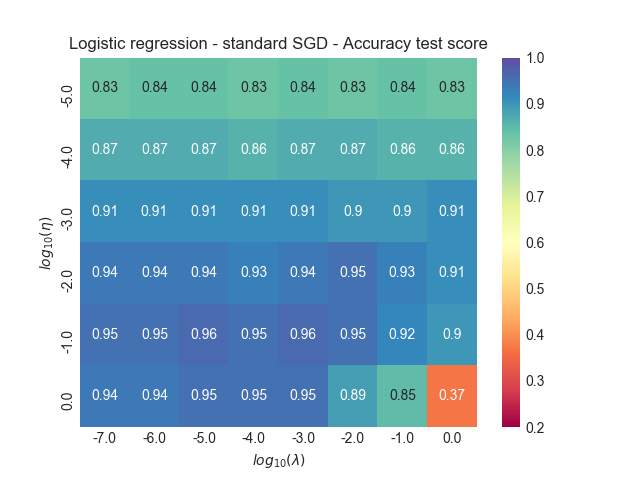
\includegraphics[width=1.1\columnwidth, height=0.65\columnwidth]{logreg_accuracy_lr_vs_lmbda_epochs=20_variant=standard.png}
        \caption{Sigmoid activation function. 1 hidden layer, 50 neurons.}
        \label{fig:15a}
    \end{subfigure}\hspace{0.1cm}
    \begin{subfigure}[b]{\columnwidth}
        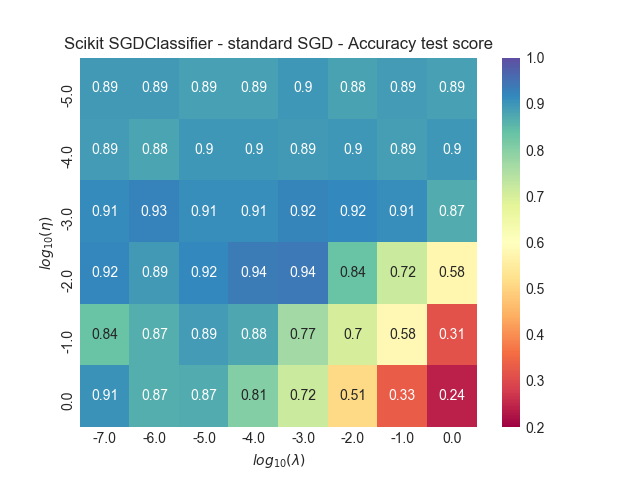
\includegraphics[width=1.1\columnwidth, height=0.65\columnwidth]{sgdclassifier_accuracy_lr_vs_lmbda_epochs=20_variant=standard.png}
        \caption{tanh activation function. 1 hidden layer, 50 neurons.}
        \label{fig:15b}
    \end{subfigure}
    \captionsetup{width=2\columnwidth}
    \caption{Figures 15 plots the accuracy test score as a function of the learning rate $\eta$ and the regularization parameter $\lambda$. Standard SGD used as optimizer with epochs $= 20$. 15(a) is results from own logistic regression. 15(b) is results from Scikit's SGDClassifier using loss="log", which is equivalent to logistic regression. All subplots have the same color-scaling range.}
    \label{fig:15}
\end{figure*}
\newpage
\section{Conclusion}
When only using the Stochastic Gradient Descent on the regression problem, we found that linear regression methods outperformed SGD. When comparing the different variants of SGD we found that due to computing an adaptive learning rate SGD with decaying learning rate, RMSprop and ADAM outperformed standard SGD. They performed better when increasing the size of the minibatches, and also converged quicker for a lower amount of epochs. For all variant, the results show a certain interval of learning rates where the error was considerably lower due to converging quickly enough but not diverging.\\
\\
Applying a neural network on the regression problem resulted in a lower error compared to linear regression methods. The reason for this is due to neural networks being more adaptable to highly non-linear functions such as the Franke function and also generalize enough to prevent overfitting. On the classification problem, logistic regression performed an par with a neural network using the hyperbolic function as activation function. Due to the classification problem being less complex compared to other classification problems, there was no benefit of using neural networks over logistic regression. When testing with different architectures, the accuracy increased as the number of neurons was increased up to a certain number where the accuracy converged. Increasing the number of hidden layers resulted in most cases a decreased accuracy due to overfitting. \\
\\
For both the regression problem and classification problem, neural networks was able to outperform or on par with simpler models but required significantly more time to train. In summary it is more beneficial, when approaching a regression or classification problem, to start out with using a simpler model/method. In some cases the simpler models are more than sufficient, but if the performance is not satisfactory then neural networks could likely be better suited to the problem.\\
\\
Possible future improvements could be to experiment more with different architectures for Feed Forward Neural Networks, for example a sparser architecture. Future ideas to try would be to use Convolutional Neural Networks on larger images with higher resolution.
\newpage
\begin{thebibliography}{9}
\bibitem{skin}
Tschandl, P. et al. (2019). Comparison of the accuracy of human readers versus machine-learning algorithms for pigmented skin lesion classification: an open, web-based, international, diagnostic study. The Lancet. \url{https://doi.org/10.1016/S1470-2045(19)30333-X}

\bibitem{project1}
Didrik Spanne Reilstad. (2020). Regression analysis and resampling methods. FYS-STK3155, Project 1. \url{https://github.com/dreilstad/FYS-STK3155/blob/master/Project1/Report/FYS_STK3155_Project1.pdf}

\bibitem{rmsprop}
Hinton, G. Lecture 6a, Overview of mini-batch gradient descent. \url{http://www.cs.toronto.edu/~tijmen/csc321/slides/lecture_slides_lec6.pdf}

\bibitem{ADAM}
Kingma, D.P. \& Ba, J.L. (2015). ADAM: A Method For Stochastic Optimization. International Conference on Learning Representations. \url{https://arxiv.org/pdf/1412.6980v9.pdf}

\bibitem{xavier}
Glorot, X. \& Bengio, Y. (2010). Understanding the difficulty of training deep feedforward neural networks. 13th International Conference on Artificial Intelligence and Statistics (AISTATS). \url{http://proceedings.mlr.press/v9/glorot10a/glorot10a.pdf?source=post_page}

\bibitem{he}
He, K. \& Zhang, X. \& Ren, S \& Sun, J. (2015). Delving Deep into Rectifiers: Surpassing Human-Level Performance on ImageNet Classification. \url{https://arxiv.org/pdf/1502.01852.pdf}

\bibitem{lrvsffnn}
Li, M. & Wang, J. (2019). An Empirical Comparison of Multiple Linear Regression and Artificial Neural Network for Concrete Dam Deformation Modelling. Hindawi: Mathematical Problems in Engineering, Volume 2019. \url{https://doi.org/10.1155/2019/7620948}
\end{thebibliography}

\end{document}
